% This is "sig-alternate.tex" V2.0 May 2012
% This file should be compiled with V2.5 of "sig-alternate.cls" May 2012
%
% This example file demonstrates the use of the 'sig-alternate.cls'
% V2.5 LaTeX2e document class file. It is for those submitting
% articles to ACM Conference Proceedings WHO DO NOT WISH TO
% STRICTLY ADHERE TO THE SIGS (PUBS-BOARD-ENDORSED) STYLE.
% The 'sig-alternate.cls' file will produce a similar-looking,
% albeit, 'tighter' paper resulting in, invariably, fewer pages.
%
% ----------------------------------------------------------------------------------------------------------------
% This .tex file (and associated .cls V2.5) produces:
%       1) The Permission Statement
%       2) The Conference (location) Info information
%       3) The Copyright Line with ACM data
%       4) NO page numbers
%
% as against the acm_proc_article-sp.cls file which
% DOES NOT produce 1) thru' 3) above.
%
% Using 'sig-alternate.cls' you have control, however, from within
% the source .tex file, over both the CopyrightYear
% (defaulted to 200X) and the ACM Copyright Data
% (defaulted to X-XXXXX-XX-X/XX/XX).
% e.g.
% \CopyrightYear{2007} will cause 2007 to appear in the copyright line.
% \crdata{0-12345-67-8/90/12} will cause 0-12345-67-8/90/12 to appear in the copyright line.
%
% ---------------------------------------------------------------------------------------------------------------
% This .tex source is an example which *does* use
% the .bib file (from which the .bbl file % is produced).
% REMEMBER HOWEVER: After having produced the .bbl file,
% and prior to final submission, you *NEED* to 'insert'
% your .bbl file into your source .tex file so as to provide
% ONE 'self-contained' source file.
%
% ================= IF YOU HAVE QUESTIONS =======================
% Questions regarding the SIGS styles, SIGS policies and
% procedures, Conferences etc. should be sent to
% Adrienne Griscti (griscti@acm.org)
%
% Technical questions _only_ to
% Gerald Murray (murray@hq.acm.org)
% ===============================================================
%
% For tracking purposes - this is V2.0 - May 2012

\documentclass{sig-alternate}
% *** CITATION PACKAGES ***
%
\usepackage{cite}
% cite.sty was written by Donald Arseneau
% V1.6 and later of IEEEtran pre-defines the format of the cite.sty package
% \cite{} output to follow that of IEEE. Loading the cite package will
% result in citation numbers being automatically sorted and properly
% "compressed/ranged". e.g., [1], [9], [2], [7], [5], [6] without using
% cite.sty will become [1], [2], [5]--[7], [9] using cite.sty. cite.sty's
% \cite will automatically add leading space, if needed. Use cite.sty's
% noadjust option (cite.sty V3.8 and later) if you want to turn this off.
% cite.sty is already installed on most LaTeX systems. Be sure and use
% version 4.0 (2003-05-27) and later if using hyperref.sty. cite.sty does
% not currently provide for hyperlinked citations.
% The latest version can be obtained at:
% http://www.ctan.org/tex-archive/macros/latex/contrib/cite/
% The documentation is contained in the cite.sty file itself.






% *** GRAPHICS RELATED PACKAGES ***
%
%\if CLASSINFOpdf
  \usepackage{graphicx}
  \usepackage{epstopdf}
 % \usepackage{auto-pst-pdf}
  % declare the path(s) where your graphic files are
  % \graphicspath{{./eps}{./pdf/}{./jpeg/}}
  % and their extensions so you won't have to specify these with
  % every instance of \includegraphics
  \DeclareGraphicsExtensions{.eps,.pdf,.jpeg,.png,.ps}
%\else
  % or other class option (dvipsone, dvipdf, if not using dvips). graphicx
  % will default to the driver specified in the system graphics.cfg if no
  % driver is specified.
 % \usepackage[dvips]{graphicx}
  % declare the path(s) where your graphic files are
  % \graphicspath{{./eps/}}
  % and their extensions so you won't have to specify these with
  % every instance of \includegraphics
 % \DeclareGraphicsExtensions{.eps}
%\fi
% graphicx was written by David Carlisle and Sebastian Rahtz. It is
% required if you want graphics, photos, etc. graphicx.sty is already
% installed on most LaTeX systems. The latest version and documentation can
% be obtained at: 
% http://www.ctan.org/tex-archive/macros/latex/required/graphics/
% Another good source of documentation is "Using Imported Graphics in
% LaTeX2e" by Keith Reckdahl which can be found as epslatex.ps or
% epslatex.pdf at: http://www.ctan.org/tex-archive/info/
%
% latex, and pdflatex in dvi mode, support graphics in encapsulated
% postscript (.eps) format. pdflatex in pdf mode supports graphics
% in .pdf, .jpeg, .png and .mps (metapost) formats. Users should ensure
% that all non-photo figures use a vector format (.eps, .pdf, .mps) and
% not a bitmapped formats (.jpeg, .png). IEEE frowns on bitmapped formats
% which can result in "jaggedy"/blurry rendering of lines and letters as
% well as large increases in file sizes.
%
% You can find documentation about the pdfTeX application at:
% http://www.tug.org/applications/pdftex

% *** ALIGNMENT PACKAGES ***
%
%\usepackage{array}
% Frank Mittelbach's and David Carlisle's array.sty patches and improves
% the standard LaTeX2e array and tabular environments to provide better
% appearance and additional user controls. As the default LaTeX2e table
% generation code is lacking to the point of almost being broken with
% respect to the quality of the end results, all users are strongly
% advised to use an enhanced (at the very least that provided by array.sty)
% set of table tools. array.sty is already installed on most systems. The
% latest version and documentation can be obtained at:
% http://www.ctan.org/tex-archive/macros/latex/required/tools/
\usepackage{balance}
\usepackage{mdframed}
%\usepackage{mdwmath}
%\usepackage{mdwtab}
% Also highly recommended is Mark Wooding's extremely powerful MDW tools,
% especially mdwmath.sty and mdwtab.sty which are used to format equations
% and tables, respectively. The MDWtools set is already installed on most
% LaTeX systems. The lastest version and documentation is available at:
% http://www.ctan.org/tex-archive/macros/latex/contrib/mdwtools

\begin{document}
%
% --- Author Metadata here ---
\conferenceinfo{International Conference on Software Engineering}{2014 Hyderbad, India}
%\CopyrightYear{2007} % Allows default copyright year (20XX) to be over-ridden - IF NEED BE.
%\crdata{0-12345-67-8/90/01}  % Allows default copyright data (0-89791-88-6/97/05) to be over-ridden - IF NEED BE.
% --- End of Author Metadata ---

\title{Experiences Gamifying Developer Practices}
%\subtitle{}
% 
% You need the command \numberofauthors to handle the 'placement
% and alignment' of the authors beneath the title.
%
% For aesthetic reasons, we recommend 'three authors at a time'
% i.e. three 'name/affiliation blocks' be placed beneath the title.
%
% NOTE: You are NOT restricted in how many 'rows' of
% "name/affiliations" may appear. We just ask that you restrict
% the number of 'columns' to three.
%
% Because of the available 'opening page real-estate'
% we ask you to refrain from putting more than six authors
% (two rows with three columns) beneath the article title.
% More than six makes the first-page appear very cluttered indeed.
%
% Use the \alignauthor commands to handle the names
% and affiliations for an 'aesthetic maximum' of six authors.
% Add names, affiliations, addresses for
% the seventh etc. author(s) as the argument for the
% \additionalauthors command.
% These 'additional authors' will be output/set for you
% without further effort on your part as the last section in
% the body of your article BEFORE References or any Appendices.

\numberofauthors{3} %  in this sample file, there are a *total*
% of EIGHT authors. SIX appear on the 'first-page' (for formatting
% reasons) and the remaining two appear in the \additionalauthors section.
%
% author names and affiliations
% use a multiple column layout for up to three different
% affiliations
\author{
\alignauthor
Will Snipes\\
\affaddr{ABB Corporate Research}\\
\affaddr{Industrial Software Systems}\\
\affaddr{Raleigh, NC USA}\\
\email{will.snipes@us.abb.com}
\and
\alignauthor
Anil R. Nair\\
\affaddr{ABB Corporate Research}\\
\affaddr{Industrial Software Systems}\\
\affaddr{Bangalore, India}\\
\email{anil.nair@in.abb.com}
\and
\alignauthor
Emerson Murphy-Hill
\affaddr{North Carolina State University}\\
\affaddr{Department of Computer Science}\\
\affaddr{Raleigh, N.C. USA}\\
\email{emerson@csc.ncsu.edu}\\
}



\maketitle
\begin{abstract}
As software development practices evolve, toolsmiths face the continuous challenge of communicating new practices and tools to the community.  In addition to training, discussing, and presenting software engineering practices and tools, we propose a method to both motivate and monitor their adoption through a tool embedded in the Integrated Development Environment (IDE).  

Blaze monitors developer practice and tool use over the long term and reports the lasting change a communication effort makes in everyday habits.  Embedding Blaze in the developer`s work environment as a Visual Studio extension captures developer work patterns while giving feedback to users on their practices.   Blaze encourages everyone to use the new practices by assigning points to specific commands and tools.  
 With a rich data source, we evaluate developer practices, define metrics that give individual feedback, and create an environment for developers to see how they are doing compared with their teammates.  

Data collected from the pilot group show a dichotomy of navigation and code understanding practices used by developers even the same developer in different situations.  We observed that the duration of an edit session is more correlated with categories of activity that benefit from improved practices and tools. The Blaze tool was well received by most participants, however, navigation practices were not significantly affected by the Blaze feedback mechanism.  We conclude that more proactive interventions are necessary to encourage developers to change their code navigation habits.
\end{abstract}

% A category with the (minimum) three required fields
\category{H.4}{Information Systems Applications}{Miscellaneous}
%A category including the fourth, optional field follows...
\category{D.2.8}{Software Engineering}{Metrics}[complexity measures, performance measures]

\terms{Human Factors, Management}

\keywords{empirical, training, learning, usability}

\section{Introduction}

Software developers who maintain code face additional challenges of navigating an existing code base to incorporate changes as they build new features or fix bugs.  Over the years, developers learn techniques to analyze code and locate areas that are relevant to an enhancment.  As new techniques and tools are introduced to the development environment, developer may not learn about them unless they interact with a peer developer who uses them\cite{wbsnipes:Hill2011Peer}.    For instance, the commands they use to navigate the code base in the development environment may make them less efficient than using newer practices or tools.  Robillard et. al. show that developers who use commands that allow them to follow code structure are more effective and efficient than developers who browse through code \cite{wbsnipes:Robillard2004How}.   

Enter the toolsmith,  who responds to challenges faced by software developers by creating tools such as code search tools that make the job easier and more efficient.  The toolsmith needs to spread the word about advanced tools they develop and determine their effect on developer practices over the long term.  Is there something we can do that encourages developers to adopt new practices and tools that also provides feedback to developers and toolsmiths on improvements that result?  

We envisioned a tool in our prior work that would motivate developers to adopt new practices or tools by providing constant feedback and allowing them to compare their improvements to how their peers are doing  \cite{Snipes2013Towards}.  This tool creates a competitive game that gives continuous feedback to the developer on adopting the improved practice.  The more they change their practices to adopt new techniques or tools, the higher they score in the game. 

Yes gamification, the incorporation of game elements into an activity that people do not typcially consider a game\cite{2013Oxford}.  Why would software developers writing serious software be interested in this?  Our first step was to challenge this question through a survey that queried both whether developers would be interested in gamifying their workspace and what aspects of that space would be most interesting to them.

With these questions answered, we identified a set of practices and defined a game meeting expectations from the developers feedback.  The game, implemented in a Visual Studio add-in called Blaze, integrates into the Visual Studio workspace and establishes a light anonymous competition between developers to improve their navigation practices. 

During the pilot of Blaze we observed the variation in developer navigation practices and identified some potential reasons for this variation.  We evaluated developer's acceptance of game elements in the tool and their desires for additional functionality.  While further data is required to assess the impact of the tool, the initial developer acceptance encourages an expanded pilot.
%state the contribution

The rest of the paper is organized as follows:  Section 2 reviews the preliminary survey-based assessment, Section 3 Discusses the design considerations for developing the Blaze tool/game, Section 4 Discusses the design of the study and participant selection, Section 5 is Related work, Section 6 results from the pilot, Section 7 Threats to Validity, and Section 8 has our Conclusions.


\section{Related Work}
%update and expand
\subsection{Monitoring Practice Studies }
Johnson and Kou defined Zorro\cite{V:Johnson2007Automated}, a system for detecting whether developers use Test Driven Development techniques based on data from Hackystat.  Zorro divides development activities into episodes delimited by events such as configuration management code check-in, start of a unit test run, or start of a build.  Using the distinct events that developers follow within these episodes, Zorro determines whether the episode followed Test-Driven Development practices per their classic definition of test first - code - test pass, or a different scenario.  In two student-based studies comparing Zorro classifications with a simultaneous observational screen video, Zorro achieved between 70\% \cite{Kou2010Operational} and 89\% \cite{V:Johnson2007Automated} accuracy in classifying episodes into their proper TDD scenarios.  The studies did not, however, attempt to use or evaluate the influence of instant feedback aimed at encouraging participants to follow the classic definition of Test Driven Development.  In our study, we attempt this leap to present data collected directly to developers attempting to influence them to change their practices.

Murphy-Hill, Parnin, and Black \cite{V:MurphyHill2012How} use the Mylyn Monitor to explore whether or not developers use the automated refactoring tools present in Eclipse.  They look for specific refactoring commands in Eclipse and determine the amount of time developers use tools versus hand refactoring the code.  For this study we build a tool that captures the use of all commands within the Visual Studio environment including refactoring, navigation, and edit commands.

Robillard, Coelho and Murphy explore hypotheses around how developers can be more effective at performing a maintenance task \cite{wbsnipes:Robillard2004How}.  Key conclusions are that developers are more more successful finding and fixing bugs when they create a detailed plan for implementing a change, use structured navigation with keyword search or cross-reference search, and only review methods once during their search.  This builds on this work by testing methods for increasing the use of structured navigation in developers` everyday practice.

The Pro Metrics (PROM) tool provides a framework for collecting data for further analysis from tools used by developers.\cite{Coman2009Casestudy}  It provides a flexible data model and a plug-in architecture to facilitate collection from different data sources.  Studies conducted using prom include a series of studies by it's creators on trends in time spent Pair Programming \cite{Coman2008Investigating}, benefits of refactoring on productivity \cite{Moser2008Case}, impact of refactoring on re-usability \cite{Moser2006Does}, and prediction of effort \cite{Abrahamsson2007Effort}.  The PROM tool and studies that use it track the time spent editing files and methods from the IDE and code metrics obtained trough source code analysis.  Applying these data to specific research questions such as whether refactoring improves productivity \cite{Moser2008Case} shows the utility of combining automated effort data with code metric data.  Taking a different focus on techniques, our study used more detailed events captured from the IDE  to detect how the user was navigating through the code in addition to knowing how long the editor is open for a particular file.

Murphy-Hill et. al. study a large usage history data set and apply several different algorithms to accurately suggest to users new commands in their environment to use.\cite{MurphyHill2012Improving} Algorithms based on command history performed well particularly when synchronized chronologically with the recipient's usage history. Novice users were better served by recommendation algorithms that did not require a long history, where more expert users benefited from more sophisticated algorithms that included more history. The "Most Widely Used" algorithm that recommends commands based on the collective usage profile of the team performed nearly as well as the more sophisticated algorithms. The paper presents the methodology for making recommendations and the evaluation of the accuracy of the recommendations. Our work goes the next step of evaluating whether a specific recommended practice gets adopted by developers when influenced through gamification methods.

\subsection{Gamification}
Singer and Schneider demonstrate the use of a message board and points for encouraging students to increase their frequency of commits to the source code repository \cite{Singer2012It}.  The communication mechanism enabled students to see each others' progress and resulted in more frequent commits than baseline.  Participants valued the communication and collaboration aspect and some valued the competition enough to change their opinion on optimum commit frequency.  The subsequent thesis by Singer \cite{Singer2013a} describes results of an experiment conducted across two iterations of a class where active feedback on commits was deployed to one course and another course served as the control group where commit frequency was simply monitored.  Results show an increase in the frequency of commits at a statistically significant level.  This study uses fine grained instrumentation to identify practices used between commits such as structured navigation.

Dubois and Tamburrelli discuss theoretical concepts behind applying gamification to software development \cite{Dubois2013Understanding}. Their approach is to consider how gamification could be applied throughout the software development life-cycle to motivate many practices in different phases.  They provide guidance on assessing gamification in the software development domain that includes analyzing the actors and game mechanics, defining integration with existing tools and processes, and designing the evaluation of results.  Dbois and Tamburrelli demonstrate this guidance using a study of students working on a class project.  Defining a control group and subject group of students, both groups receive the same feedback about their code comments, test coverage, code size, and static analysis rule violations.  The subject group can see each others' rankings while the control group only sees their personal rankings.  Results though inconclusive indicate that competition increases the desired results.  In our study we apply both individual feedback and competitive based feedback (anonymized) to participants and seek to observe a change in their behavior after an intervention.

\section{Pre-study Sruvery on Viability of Applying Gamification for Software Engineering}

\subsection{Pre-study Background}
When discussing gamification, folks raise a concern about replacing an activity that is intrinsically motivated with extrinsic motivation provided by points and achievements.  To discover what is behind this concern, several studies are useful to understand what should be done. 

Early studies attempt to evaluate achievement motivation in students and relate that to their performance in school.  The study by Hermans describes results from applying questionnaire to evaluate achievement motivation in students \cite{wbsnipes:Hermans1970Questionnaire}.  Each question is ranked for its correlation to achievement motivation. Some key questions about the diligence with which students approach their work are correlated with achievement motivation.  

Maehr proposes an affirmative theory whereby  individuals achieve as a member of a social group choosing the behavior that will meet the expectations and values of the group that is significant to them \cite{wbsnipes:MaehrCulture}.  The presence of a social group where the person is motivated to belong and excel within is important for creating achievement motivation.  Maehr states that since achievement behaviors can be triggered by circumstance, that they are present in most people regardless of background. 

Beecham and colleagues provide a thorough analysis of existing literature on studies of motivation in Software Engineering \cite{wbsnipes:Beecham2008Motivation}. It has some valuable lists of factors that motivate software engineers with the most common being ''the work'' motivates us. The list of de-motivators is also useful with common job satisfaction items like stress and inequity in recognition, plus poor quality software (low accomplishment) and lack of influence in decision making. The paper also lists characteristics of people in the professions including need for independence (autonomy), desire to learn new skills/tackle challenges. 

Understanding the concerns with maintaining intrinsic motivation while adding elements of achievement motivation, we developed an assessment survey questionnaire to determine whether the community would be receptive to a gamification approach to software development.   We designed  the survey to assess how developers are motivated to use training, practices, and tools and whether they are open to having that information shared with their peers and managers, and being recognized with badges and points. The developer study conducted with over 130 software developers at ABB challenged whether achievement motivation would help software engineers and whether they would accept sharing data on tools and practices they use to help others.

\subsection{Pre-study Survey Results}

Using a question from the Saachi and Saachi survey \cite{wbsnipes:SaatchiGameification} as directly as possible, we asked developers at ABB "How interested they would be in working for a company that incorporated some aspects of games into software engineering tools as a way to increase productivity in the workplace"?  We segmented results by country in Figure \ref{fig:gamification} and found that gamification of software engineering is more interesting to developers in India, Poland, and Finland than in other major countries.  The responses indicating that developers were at least somewhat interested is 75-88\% In India, Poland, and Finland.  For the US, Sweden, and Switzerland the responses indicate 60-65\% are at least somewhat interested.  The overall response from our survey is comparable to the Saachi and Saaschi survey\cite{wbsnipes:SaatchiGameification} upon which this question was based that found 75\% of 18-45 year olds were at least somewhat interested.  
%EMH why is our survey result comparable to Saatchi?
\begin{figure}
	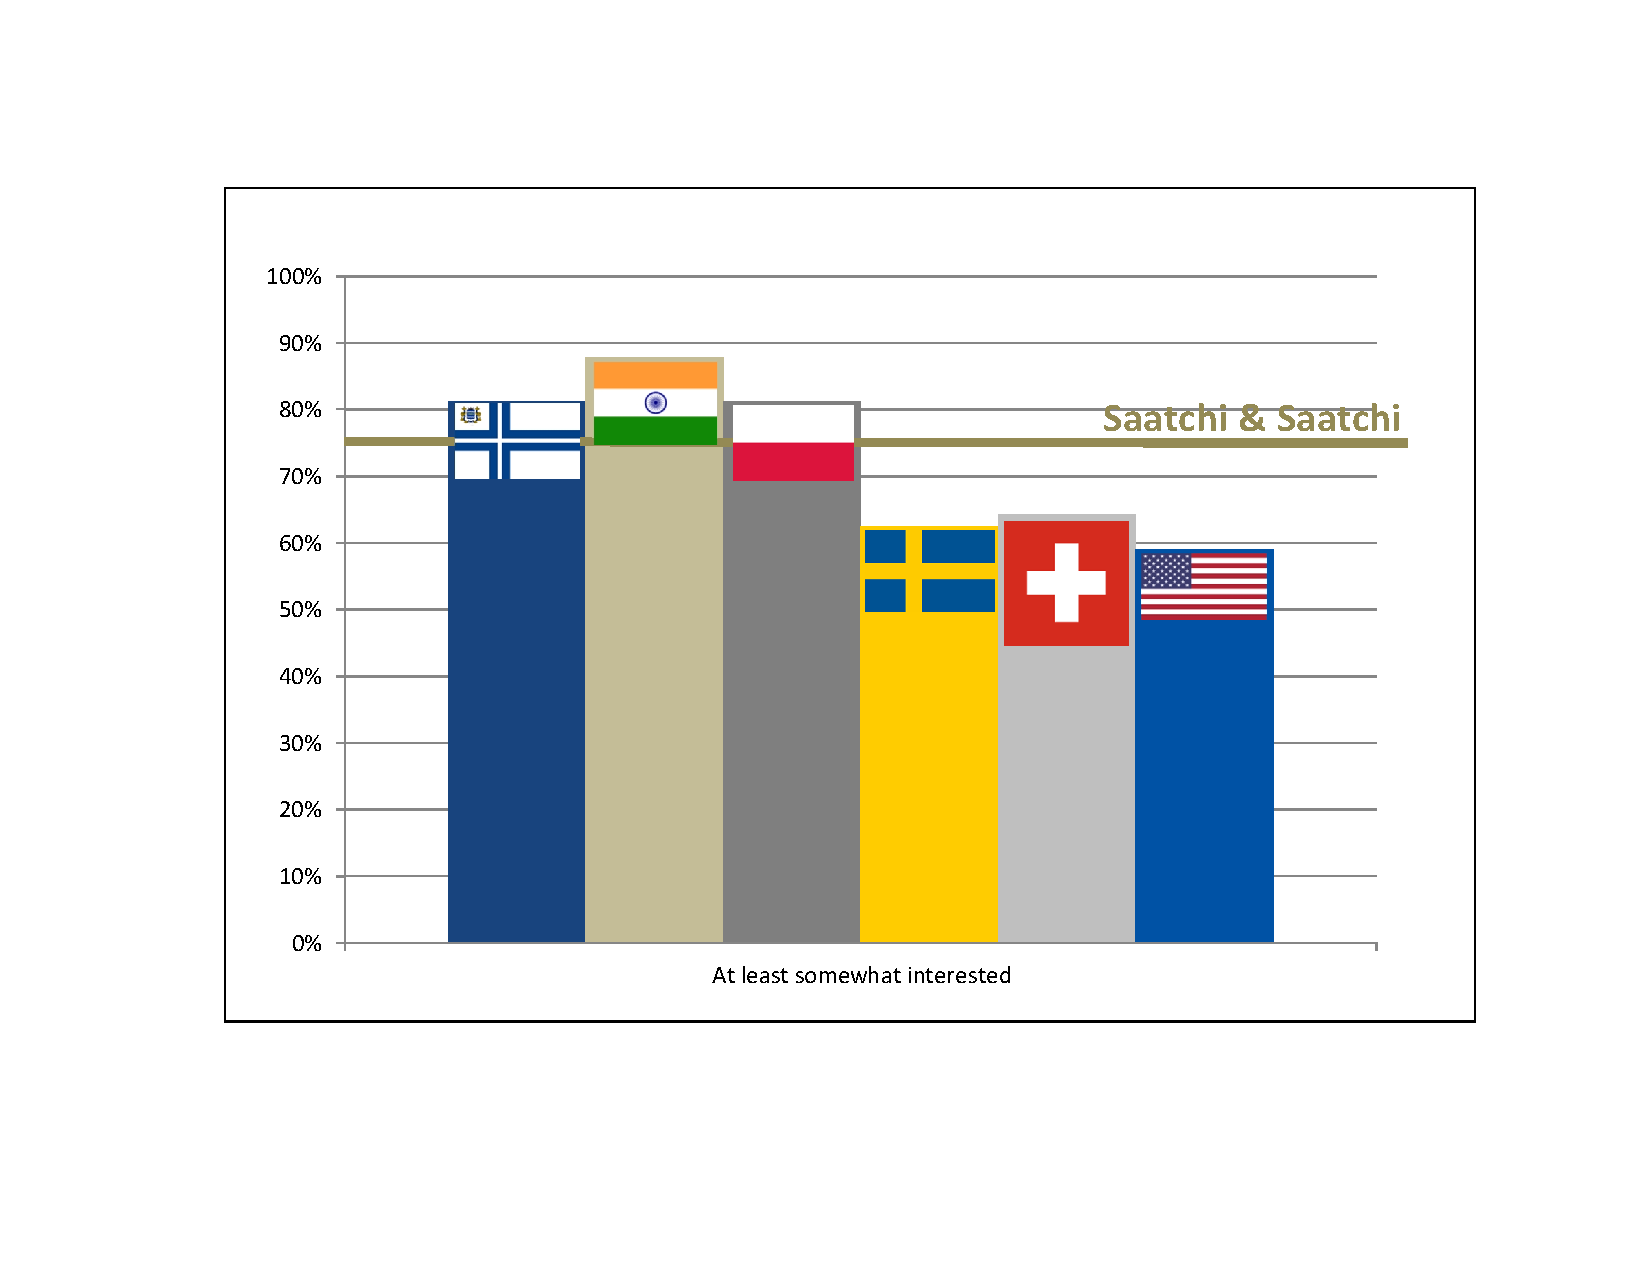
\includegraphics[width=3.4in]{gamificationquestion.pdf}
	\caption{Acceptance of gamification}
	\label{fig:gamification}
\end{figure}

We asked developers how likely they would be to try tools and practices recommended to them through an automated usage tracking system.  Answers showed that 95\% of the developers surveyed are likely to try the recommended tools and practices.  This indicates that a recommendation system would positively impact the deployment of software engineering tools and practices at ABB.

Another question was whether sharing detailed usage information with colleagues and the company as a whole would be a concern for developers.  A graduated scale was used for the community that would be shared with and distinction between whether that sharing was anonymous or the information was personally identifiable. Figure \ref{fig:comfortwithsharing}  shows that over 90\% of respondents are comfortable with sharing either anonymous or non-anonymous information with their team members. 
Their comfort level decreases as the scope of who the information is shared with increases.  People were less comfortable sharing with anyone (the category for people outside ABB) particularly if the data were not anonymous.  
Two conclusions from this feedback are that people are very willing to share information that could help their team. Second, sharing within the company is acceptable if we take care to make the data anonymous.

\begin{figure}
	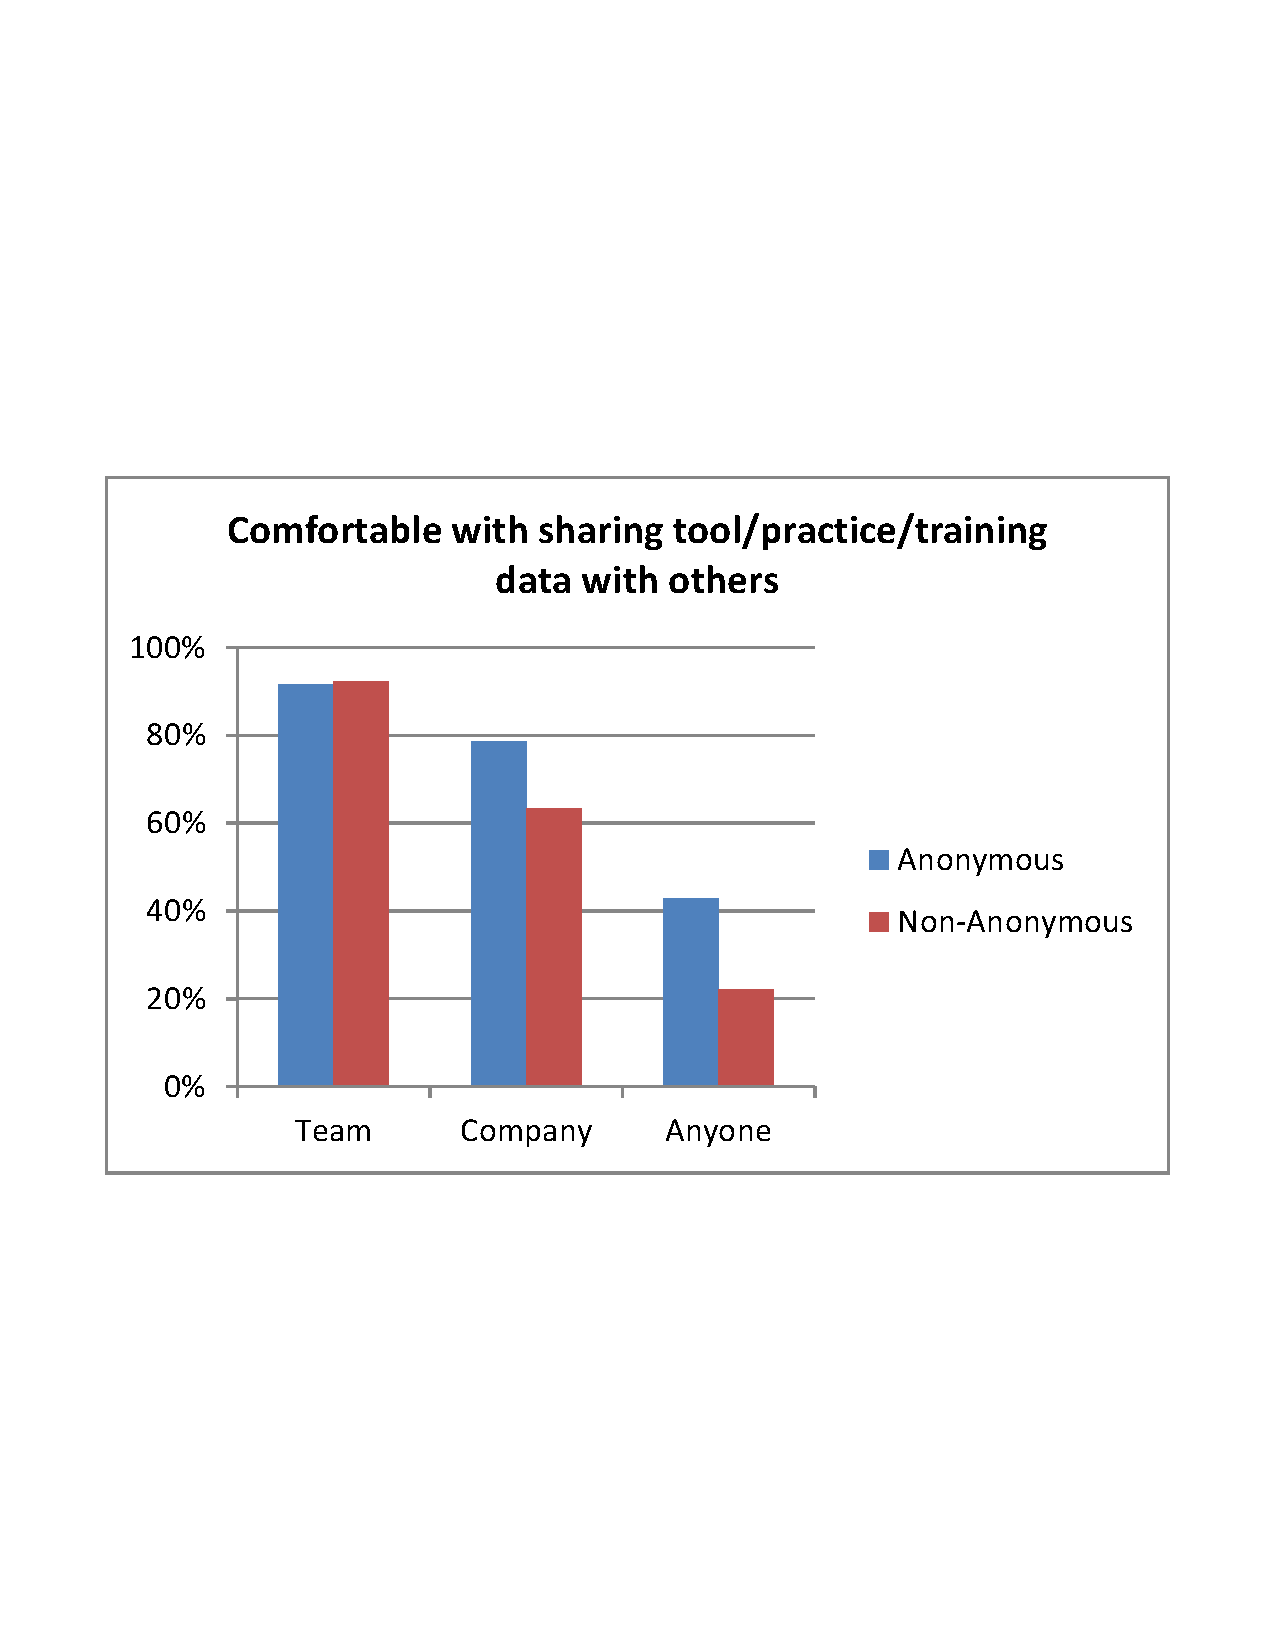
\includegraphics[width=3.4in]{ComfortWithSharing.pdf}
	\caption{Comfortable with sharing usage information}
	\label{fig:comfortwithsharing}
\end{figure}

Developers were asked what would motivate them to use tools and practices and given 4 choices to rank.  The top motivator for using tools and practices is coworker recommendation with 75\% of respondents in Figure \ref{fig:toolandpracticemotivators}   ranking in 1st or 2nd place. The lowest was having badges posted on their social profile where 33\% ranked this in 1st or 2nd place.   Badges also ranked low in motivations for taking more software engineering training.  We conclude that a facility to share coworker recommendations on tools and practices has the best opportunity to increase their adoption.  Since a competition among teams ranks slightly higher than management mandate, we have the choice to apply one or the other or both as motivation for using key practices.  
 
\begin{figure}
	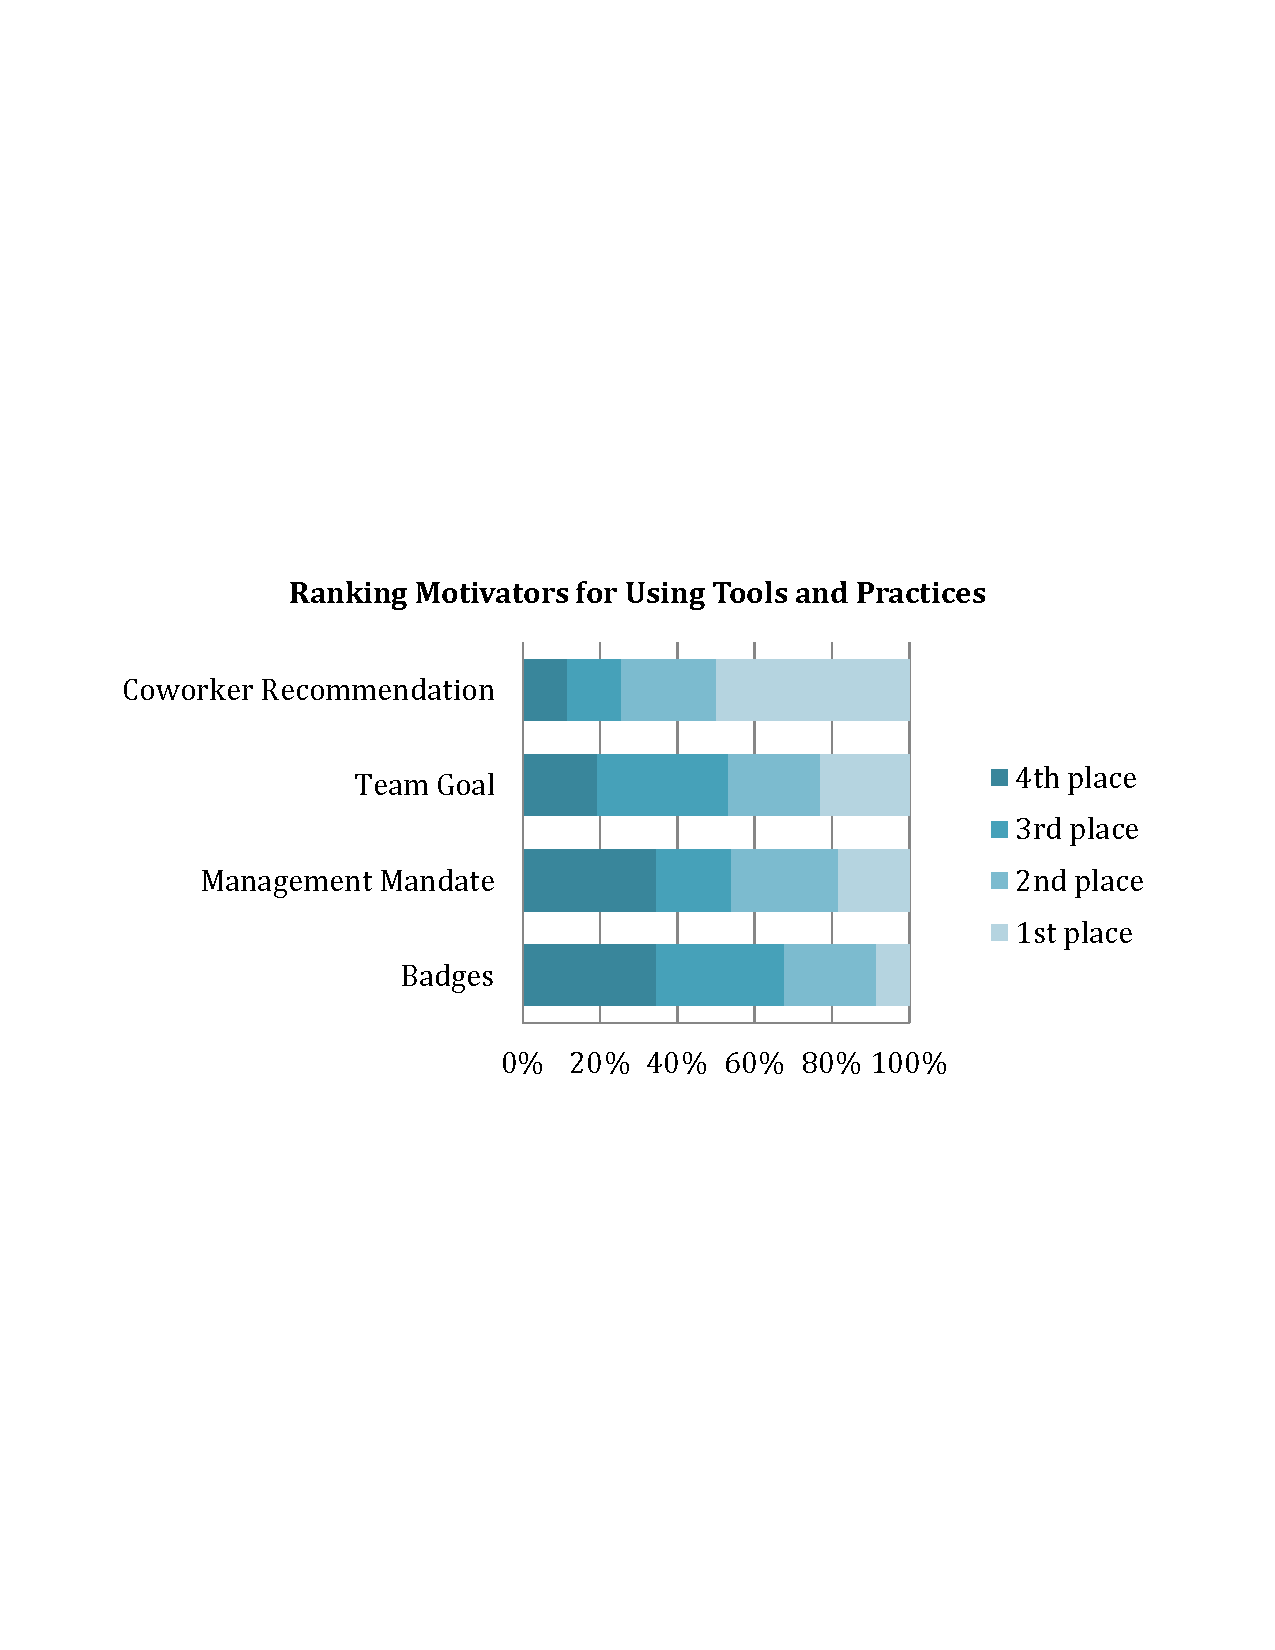
\includegraphics[width=3.4in]{ToolAndPracticeMotivators.pdf}
	\caption{Motivation for using tools and practices}
	\label{fig:toolandpracticemotivators}
\end{figure}

Developers were asked to rank awards for different actions by which they would find the most desirable.  Overall 68\% of developers ranked receiving an award for consistently performing quality practices as either 1st or 2nd place.  This supports a conclusion that focusing on awarding quality practices would motivate developers to do them consistently.
%EMH connection?
\begin{itemize}
\item 95\% of developers responding would try tools and practices suggested by an automated recommendation system particularly if they were provided in context with the current work-flow pattern the developer follows.
\item Responses indicate a preference for team competition over individual awards (badges) and awards for quality practices ranked highest.  So, the tool will incorporate team competition ideas and recognize quality practices.
\item Over 90\% of respondents approved of sharing data with their team members
\end{itemize}



\section{Game Design}

%\begin{enumerate}
%\item Define the practice we wish to measure compliance with
%\item Develop a mapping of the practice to actions that are captured by the blaze tool from the IDE
%\item Weight the actions according to their importance to the practice and assign points to the actions in the configuration file
%\item Develop the intervention method
%\item Determine the phases and length of the phase in the study according to baseline, intervention, and continuous feedback
%\item Select participants to deploy
%\item Define a pre-study questionnaire if one is necessary to collect associated information
%\item Define a post-study questionnaire if necessary to collect post study information
%\item Communicate with the participants about the study
%\item Execute the study and report results
%\end{enumerate}

%distinguish pilot from pre-study.  How does gamification apply?
The pilot evaluates the aspects of game implementation as well as the study of the results of their results. Here we discuss how the aspects of selecting a practice suitable for gamification, designing the game, and competitive element considerations.

\subsection{Select a Practice}
%transition
In their paper on game design patterns, Hamari et. al. issue a warning that assigning achievements to required tasks reduces intrinsic motivation because player autonomy is reduced by the achievements \cite{wbsnipes:Hamari2011Framework} .  This warning indicates that we should avoid giving points for things that are already an expected deliverable such as finding or fixing bugs, completing development tasks, or meeting required process criteria.  
%passive
Practices to consider are those practices with room to go beyond a checklist or minimum criteria where developers have the opportunity to excel.
%passive
Selecting a practice to study involves identifying a practice, defining specific characteristics of the practice to measure, and identifying the actions in Visual Studio that relate to the practice.  We currently limit ourselves to practices that exist entirely in the IDE thus can be monitored using Blaze.  We identified potential practices of test-driven development, debugging practices, navigation practices,  eliminating static analysis bugs, and check-in frequency.  
%EMH is check-in frequency a practice?
Practices of check-in frequency, static analysis bug elimination are highlighted in this paper's related work section with prior gamification studies in classroom environments.  Johnson and Kou achieved automated monitoring of test-driven development practices with Zorro thus may provide a candidate for future gamification application.   
%reference
Debugging practices have developer community opinions on optimal methods, however, detailed debug practices with modern IDEs have not received research community attention, thus are also reserved for future work.  

Based on studies of structured navigation by Robillard et. al. that identify structured navigation as a practice leading to effective program maintenance  \cite{wbsnipes:Robillard2004How}, we identified structured navigation as a key practice.   Structured navigation fits the requirement of a practice that is contained in the IDE, is something that has proven benefits, and lends itself to measurement and scoring, is not an assigned task, and leaves room for developers to excel.  

\subsection{Design the Game}

To setup the game for a practice, the Blaze tool provides an XML configuration file where the researcher can configure Blaze to categorize and assign points to the commands that are part of a software engineering practice.  Blaze allows the researcher to define multiple command category levels.  Thus we can categorize commands that are navigation then further classify them into structured and unstructured navigation.  

We categorize commands as structured navigation when they allow the developer to locate a code element following the program structure from another element.  For example, Navigate To \textit{Ctrl+,}, Go To Definition \textit{F12}, and Find All References \textit{Ctrl+K,R} are commands that follow structure of the code, which we classify as structured navigation.

Commands that we considered as unstructured navigation include scrolling through a file using keys or the scroll-bar, opening files from the Solution Explorer, Find commands (e.g. Find in Files), Go-to line number, and children of these commands (e.g. Find Next).

To evaluate developers using recommended tools in Visual Studio, we categorized them by their tool name.  In the pilot we were interested in developers learning about and using the Sando search tool.  Sando is part of the recommended developer tool suite for ABB and supports structured navigation using code search \cite{Shepherd2012Sando}.

Gamification practices consider the feedback of achievements and points as critical to a successful outcome.  The design of achievement awards should gradually encourage the participant to reach higher and higher levels of success in the activity.  Achievements must feel earned to the participant so that internally they recognize the effort to get the award was significant and feel satisfied  \cite{wbsnipes:Hamari2011Framework}.  Hamari and Eranti describe a general relationship between achievements in games and regular game play      In games achievements are typically a parallel scoring system to the main game play.  They make the game more engaging providing multiple ways to increase your score and multiple challenges in one interface.

Using these guidelines we assigned points to structured navigation commands which received 1 point each while unstructured navigation commands received 0 points.    We gave additional emphasis to using the Sando search tool by assigning it 10 points.  In creating levels, following the guidance from Hamari \cite{wbsnipes:Hamari2011Framework}, we built levels following an exponential curve.  Users initially level up after a working day or two extending to achieving the next level after a week or even a month following an exponential curve.  The levels make the game motivating for beginners and challenging for more experienced developers.  We designed the points and levels such that above average developers can complete all levels during the study period.


\subsection{Competitive Elements}
By selecting an intact team, we hope to leverage aspects of motivation such as the Leaderboard to spur feelings of competition among teammates.    The leaderboard was presented so that developers could see their own score in relation to the top 5 people on the leaderboard.  However, the identifier of the other participants was generated as 3 capital letters assigned based on their position on the leaderboard.  Therefore the assigned letters could even change when an individual's ranking changed.  Not knowing who of your colleagues was ahead of you could be a factor in motivation, but also avoids one potential source of conflict in an intact team.

Competitive dynamics may be more effective when teams from different areas can compete as a team against other teams..  This tried and true method both builds esprit de corps and enhances achievement towards the intended outcome.  This study design is potential future work. 

\section {Study Design}

Utilizing the unobtrusive continuous monitoring capabilities of Blaze, we designed the pilot to reveal feedback to the developer in 3 stages of 1 week duration each.
% Longtiudinal studies allow us to design an experiment and determine the effects over two or more sample periods using standard MANOVA (Multiple ANalysis of VAriance) models. \cite{longitudinalbook}  
We employed the three stage model defining the first stage as a baseline capturing the current practices of the pilot group.  The second stage employed the intervention that included an informative web site on structured navigation commands in Visual Studio, information about the Sando search tool, and information about how points would be awarded during the pilot.  The third stage provided the participants with continuous feedback in the from of points accumulated and an indicator arrow that points up when their navigation ratio is higher than their historical average.  

\subsection{Intervention Staging}

Part of the research objective was to determine whether we can achieve adoption of a practice with alternative interventions that are more deliberate than word of mouth and perhaps more scalable than webinars or presentations.  As previously discussed we sought to provide Blaze as a means to influence developers to use structured navigation practices.  We constructed the interventions during the pilot to roll out in stages each week that they use the tool.  This allowed us to establish a baseline and determine the changes as the pilot continued.

In the initial stage, participants were informed of the purpose of the study what to expect from the Blaze tool.  The participants installed the tool in their Visual Studio environment.  The tool did not present any window for them to see and simply collected data in the background.   

After a week's data collection marking the end of the first stage, Blaze started to automatically pop-up a window containing a button for a web page with information.  The page included a link to download Sando  and information about using that tool in a video.  The sub-page on navigation contained a page of tutorial on the built-in structured navigation commands in Visual Studio.  The About Blaze page contained details of the point scoring system and background on Blaze's purpose.  The usefulness of the communication site is rated as part of our study completion survey.

In the third stage developers received instant feedback from Blaze on the points they accumulated during the development session.  The up/down arrow provided a simple indicator on whether they were increasing their use of structured navigation or were using it less than their personal historical average.  This final configuration continued until the end of the pilot.  

\subsection{Pilot Participants}

As mentioned in Figure \ref{fig:gamification}, India is one country where as per our survey, the acceptance to gamification is the highest. Hence, we conducted this study with an intact team of 6 developers working in an R\&D facility in India on a large industrial software system. We approached a team which develops and maintains an industrial software product. Initially, we met the whole team along with the management staff to explain the research project and the Blaze tool we developed. We  explained the aim of the study, what data is collected, and how the data will be processed and managed. 

It was important to gain the confidence of the participants that their data were kept confidential so their activities would be close as possible to real-world. if the participants felt like they are being tracked and the data is going to use for some study that would identify them to their peers or managers, then they may deviate from the natural development style.

We  assured the team about the confidentiality of the data and the management also informed the team that the data collected by the research group will not be used for any other purpose other than the study.  Developers were asked to volunteer for the pilot by their management, however, managers did not know who participated in the study. Their name and data were kept confidential to ensure that no one apart from the research team knows that he/she is participating in the pilot. Mechanisms in our data collection to identify individuals were under the control of each developer, they could chose to share or keep confidential the association of a generated unique id with researchers or each other.   

Management wished to have no knowledge of who was participating and took great care to remain detached from the pilot proceedings.  Data at this level of detail has not been collected in ABB development organizations except for a few minutes of video study that might be conducted.  Researchers were careful to create the system so that developers controlled their identification with the data and fortunately, management bought into the necessary anonymity of the participants.
%Through this approach, we ensured that the developers are performing the task on a very natural environment with out bothering that they are being tracked.
\subsection{Pilot Survey}

The goal for the pilot follow-up survey was to collect feedback on the tool and the effect it had on the developers` navigation practices and knowledge.  The survey questions were segmented into portions that evaluate prior and post knowledge and practices for navigation, key steps in the pilot itself, the influence of game elements on their navigation practices, typical tasks and demographic information.

The key questions about this pilot were did we have an effect on knowledge of the developers regarding structured navigation commands.  We asked them to rate their knowledge of structured navigation commands prior to the pilot on a 1-10 scale to understand their baseline.  We asked them to contrast their knowledge after the pilot to assess what they learned from the pilot.

The other key question is did we have an effect on their navigation practices.  Here too we asked them to rate how much they used structured navigation prior to the pilot using a 4 choice rating of not at all, some, many times, and as much as possible.  Then we asked whether the used structured navigation commands about the same amount, more,  or a lot more during the pilot.  These two questions assessed their intent in terms of using structured navigation commands and we checked that with the data.

A key set of questions focused on whether using Blaze increased their attention to navigation commands by asking how much specific game elements influenced their practices.  The scale started with not at all, a little, some, to a lot.  

The other questions included whether they reviewed the training materials on structured navigation commands, installed the Sando code search tool, and what types of development tasks they would consider using structured navigation for in general.  Another demographic question is how well they know the code they work in rated from "I work in code that I wrote", "I maintain code that I am familiar with", to "I recently learned the code"

\section{Results}

\subsection{Pilot Data Observations}

Blaze logs events from actions the developer takes or actions from Visual Studio itself.
 The event is basically a GUI event that the program manages with event handlers that are registered with the application to listen for the event.  Blaze becomes a global event handler listening for all events by registering for them in Visual Studio.  

Blaze records key attributes along with each event in visual studio.  The log captures a time-stamp for each event normalized to GMT.  The name of the event provides a low-level classification.  The event type reflects an internal classification in Blaze.  An optional field for Artifact Reference captures data such as the file-name being edited and the currently selected line number.  Finally an anonymized unique identifier for the user of blaze allows us to investigate differences between developers.

Analysis of the log extracts several key information bits from this raw source.  First we classify the event names at a higher level into categories related activities such as Navigating, Reading, Editing, Building, Debugging,  Testing, and using a  known Tool.  

The second information we extract is aggregating the events along the time-line into sessions.  A session is an abstract concept that groups multiple events into a sequence with a beginning and an end.  Of the many possible ways to define sessions, we chose to define sequences as all the events that transpire before and during a set of edits to a specific file.  When the developer edits a new file, all the events after the last edit to the previous file are part of the new sequence for the new file.  Although not at the method level, this is similar to the say Robillard et. al. generated sequence based on located methods for their study.\cite{wbsnipes:Robillard2004How}

%\subsubsection{Observations About Developers` Habits}
%
%We are interested in understanding whether developers are consistently using practices that make them inefficient.  One way to check that is to determine whether our measurements are associated with specific developers in the study, in other words, can we independently classify the edits performed by each developer.  If this is possible, then we can discuss whether developer have consistent ways of navigating and understanding for each edit.  Thus the hypothesis is developers have consistent ways of navigating and understanding code while they are making changes.
%
%To test this hypothesis we construct a classification tree using Weka \cite{Hall2009WEKA} with the J48 classifier.  Slicing the data and training the model using 10-fold cross-validation, the model identifies 53\% of the 647 edit sessions with the correct developer among 6 participants.  The tree uses nearly all available fields including time for all categories and time of day for edits in its attempt to associate sessions with their developer generating a Kappa statistic of 0.403  and square root of the relative squared error at 101\%.  
%
%While there is some consistency to how developers work, we cannot say that individual developers are always consistent in their work patterns.  Thus developers are somewhat flexible in the commands they use when navigating and making changes to code and may be more open to adopting new tools and techniques.\

\subsubsection{Observations About Drivers of Edit Session Duration}

We selected navigation as the subject of the pilot game because it was identified by Robillard et. al\cite{wbsnipes:Robillard2004How} as correlated with developers who effectively completed a maintenance task.    Are we focusing on the right area of developers` activity in Visual Studio?

In order to test whether navigation is an important area to address, we construct a hypothesis that use of unstructured navigation is an important factor in developer productivity.  Edit session duration, we assert by opinion, is a factor related to developer productivity though there are many other factors we could consider.  With the data available from Blaze, we can explore the categories of events that correlate with the duration of edit sessions over the period of the pilot.  

Using Weka\cite{Hall2009WEKA}, we performed an attribute selection process to identify the most significant attributes related to edit session duration.  The attribute search method we chose was Greedy Step-wise search that selects attributes based on their correlation with the target and stops adding attributes when the next attribute decreases the correlation.    The process identified the top 5 out of 15 possible categories as follows:
\begin{enumerate}
\item Unstructured Navigation
\item Debug - events from running the debugger
\item Edit - events that modify the code
\item Other Actions - other events in visual studio that we do not sub-classify
\item Build - events from running a build
\end{enumerate}

Using R\cite{Rcitation}, we constructed a linear regression model for Unstructured Navigation to determine the correlation with edit duration.  The linear model found a positive correlation with unstructured navigation with a p-value <0.001 on 1694 degrees of freedom.  The model had an Adjusted R-squared of 0.64 showing a good portion of the variation in edit duration is explained by that category. 

This analysis shows that we cannot disprove that unstructured navigation is correlated with edit duration, thus it is an important factor in developer productivity.  Combining unstructured navigation with reading describes a larger portion of the overall edit duration and motivates us towards making tools that improve both navigation methods and code comprehension.  

\subsubsection{Observations on Navigation Ratio}

To evaluate whether developers improved their practices for structured navigation we established a metric Navigation ratio as the number as the number of structured navigation events in a session or period of time over the number of unstructured navigation events.  

Structured navigation events included: 
\begin{itemize}
\item Navigate To (Ctrl+,) is a fuzzy search interface that locates symbols matching your search terms.
\item Go To Definition (F12) brings up the code where the selected symbol is defined. 
\item View Call Hierarchy (Ctrl+K Ctrl+T) provides a two way analysis of a symbol's dependencies and uses. 
\item Class View (Ctrl+W, C) provides a browser and search function for classes and class hierarchy
\item Find All References provides a list of references for an object
\item Navigate to Event Handler brings up the event handler from the XAML editor
\item View Class Diagram generates a class diagram for the project
\item View Object Browser is a search tool for objects in the solution
\end{itemize}

Unstructured navigation events included selecting a file in an explorer window or selecting the tab for a file, using arrow and page up/down keys to go up/down through a file, scrolling, clicking on a file element, and using any of the built-in find commands such as Find In Files or Quick Find.

During the pilot we staged the deployment of information feedback to developers so they would first have access to learn about structured navigation and then get instant feedback in the form of points for using structured navigation commands.  Our hypothesis was that this instant feedback and information would result in an increase in the number of structured navigation commands used in Visual Studio.

To evaluate whether developers use more structured navigation when they receive instant feedback, we monitor the change in navigation ratio over the pilot study period.   Expecting that as developers learn about navigation commands and tools that count towards the score in the second week they will begin using the practices more.  In the third week we turn on points feedback and the leaderboard expecting this will encourage developers to use more structured navigation.  

\begin{figure}
	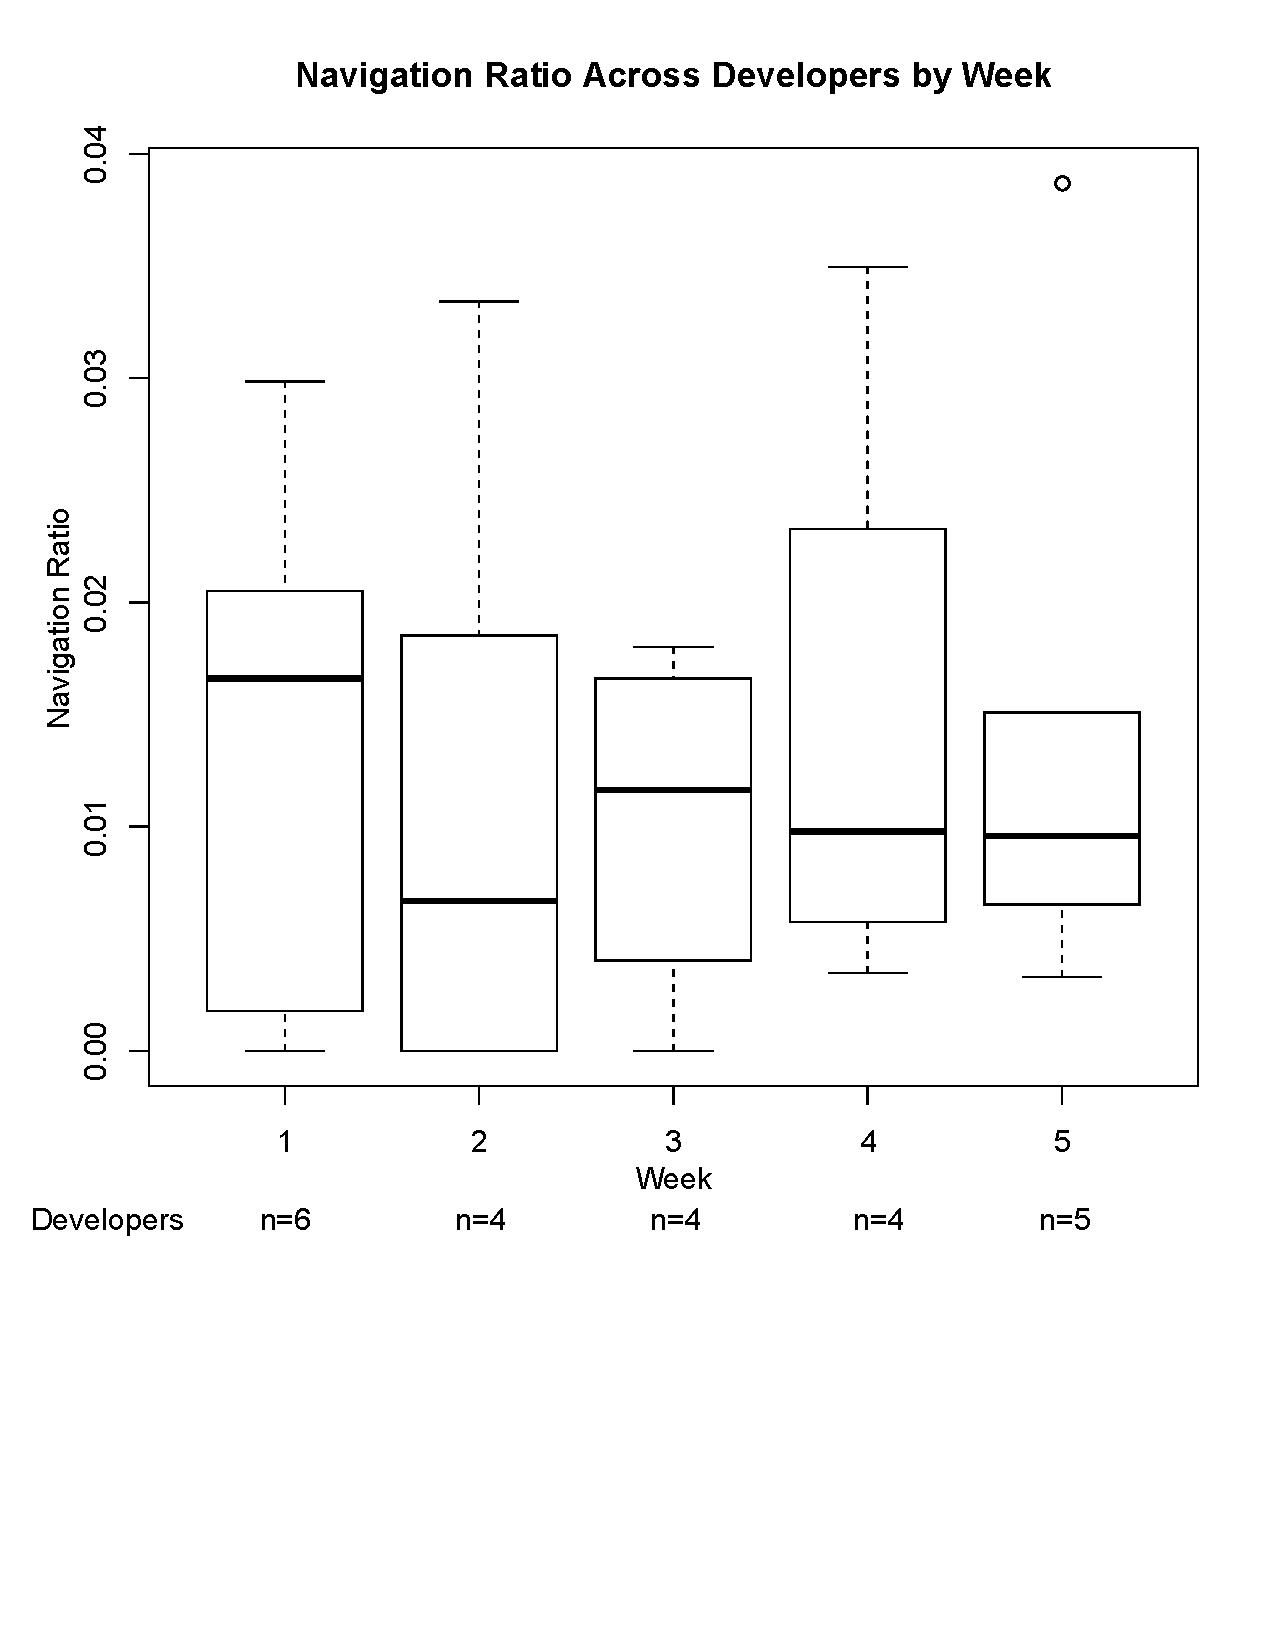
\includegraphics[width=3.3in]{navratioboxplot_ann.pdf}
	\caption{Navigation Ratio by Week}
	\label{fig:navigationaverage}
\end{figure}

What we observed visually in Figure \ref{fig:navigationaverage} is that the structured navigation practice did not increase significantly from the beginning to the end of the study.  We evaluated the week over week differences using a Wilcoxon Rank sum test that compares week one to week two and week one to week three.    In week two when the developers were able to learn about structured navigation commands there was no significant change.  Also in week two, two developers stopped participating, one was working in another environment and the other dropped of for the rest of the study.  Week three there was a slight increase, however the increase is not significant.  Weeks four and five that follow the formal period of study show the navigation ratio continues in a similar range.  Overall, we did not see a significant effect towards increasing navigation ratio for the interventions Blaze provided to the environment. 

\subsubsection{Observations on Points}

The developers using Blaze received feedback in the form of points given for using structured navigation commands and using the Sando search tool\cite{Shepherd2012Sando}.  Per the pilot design, the points display was disabled until the third week following installation so that a baseline without instant feedback could be established.  The points display and the navigation arrow were enabled in the third week to test whether the instant feedback was successful in driving increased use of the targeted features.  Observing the result shows that during the first two weeks, we see in Figure \ref{fig:pointsbyweek} developers were fairly consistent in their use patterns.  With the introduction of the points feedback, two developers` points accumulation spiked in week three due mostly to increased use of Sando.   We informed developers at the beginning of the pilot that Sando usage would receive 10 points and using built-in structured navigation commands would receive 1 point.

\begin{figure}
	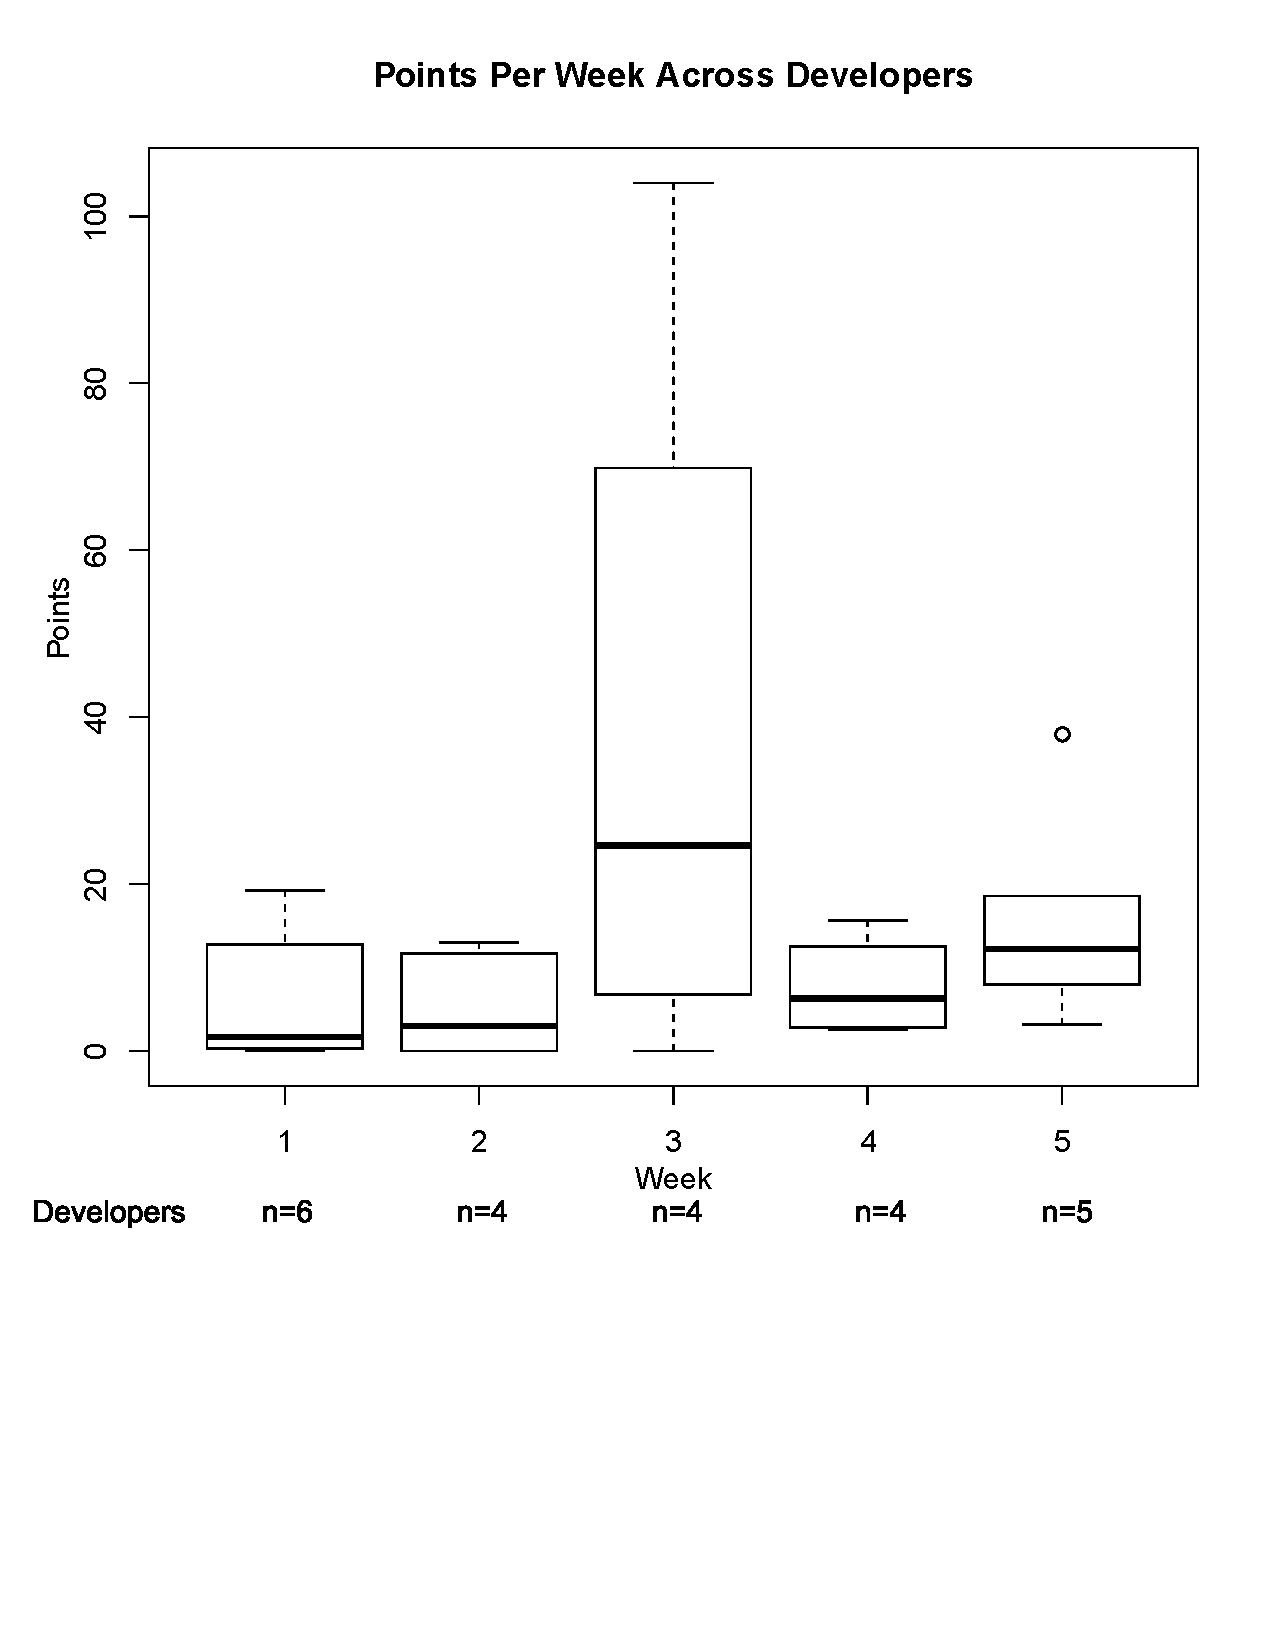
\includegraphics[width=3.3in]{pointsbyweek_ann.pdf}
	\caption{Average Points per Day by Week}
	\label{fig:pointsbyweek}
\end{figure}

\subsubsection{Direct Feedback Discussions}

\begin{figure}
	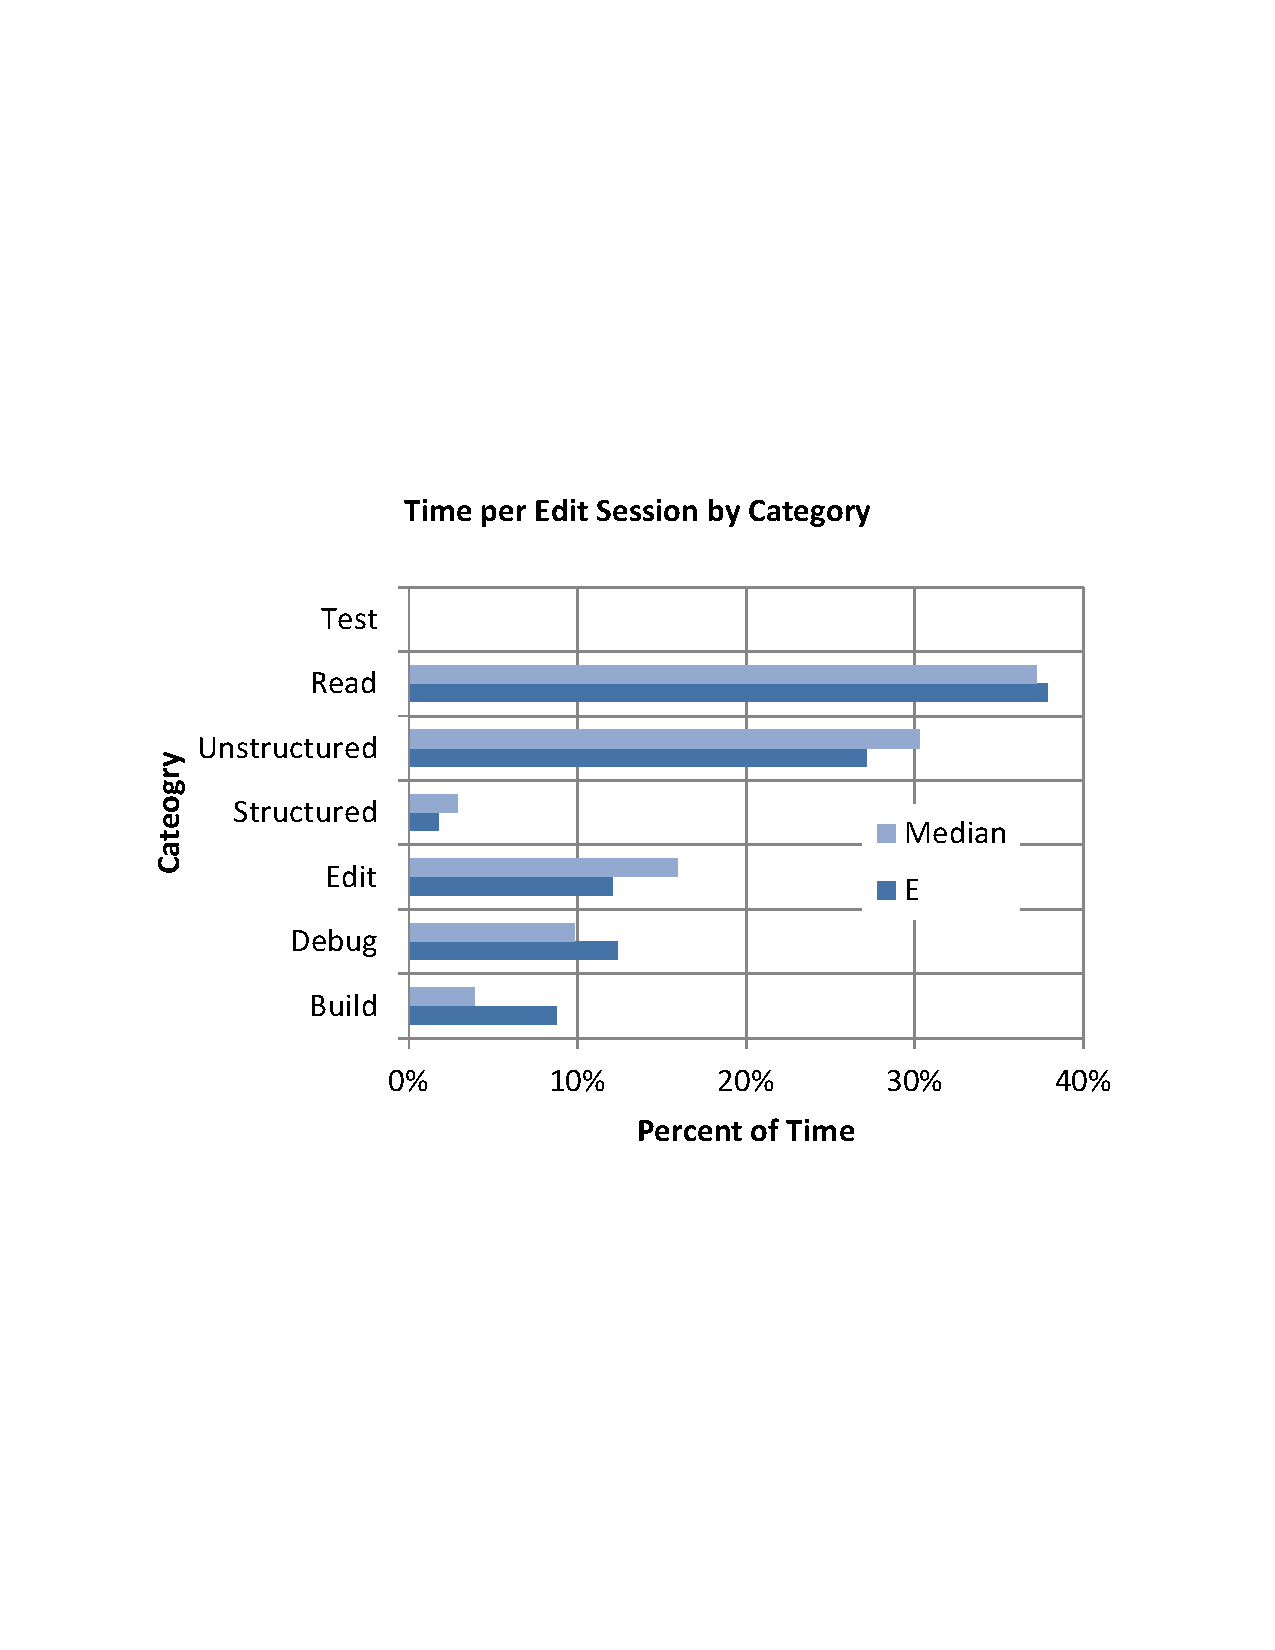
\includegraphics[width=3.3in]{developerEmedian.pdf}
	\caption{Developer Analysis Against Median}
	\label{fig:developercomparison}
\end{figure}


Following our data analysis, we conducted one on one feedback sessions with the pilot participants. Before initiating the discussion, we assured the individual developer that the data shared with them is confidential and we will not share the same with management. The participants received the feedback in the form of quantitative charts and written analysis of the information.  The key quantitative chart shown in Figure \ref{fig:developercomparison} compared their distribution of time in each category to the median for the group.   

We discovered during these feedback sessions that developers did not spend the entire time in their desktop environment because they had a virtual machine environment available for testing. Thus categories like testing, debug, and reading were affected by whether or not they used the virtual environment or their desktop for these activities.  Individual differences in those categories are considered irrelevant and not discussed here. Because our game points analysis focused on navigation commands excluding reading, the presence of the virtual environment may explain how the data have missing values on some days.  

We also discussed with one developer who`s build effort and the underlying build frequency was much higher than median as shown in Figure \ref{fig:developercomparison}.  We asked the developer to explain how building more frequently helps them. The developer mentioned that by doing more frequent build, (s)he is trying to ensure the correctness of the work completed so far. The developer feels that if (s)he resolves the bugs then and there, (s)he can do it faster as the code and logic is fresh in her memory. If they build less frequently, even though it reduces the build effort, there are more bugs each time and the developer often spends more time in identifying the problem area than fixing it. Hence the developer feels that more frequent builds improves their productivity.  

In another case, we observed a higher level of unstructured navigation than median and asked the developer about that.  They explained that even though they agree that structured navigation is better than unstructured navigation, (s)he prefers unstructured navigation in some specific instances. The developer is the author of the code and (s)he knows the code completely. ``I know that the line I need to fix is in XYZ method and it is 4 blocks down from where I am currently. It takes much less time for me to reach the fix location using unstructured navigation. If the code is not written by me, I will prefer structured navigation.'' This instance cautions us to gather information on aspects such as code familiarity and developer experience with the product when assessing the results of a navigation study.


%Though commonly held opinion of Microsoft`s Clippy experience suggests this more invasive form of feedback is not always welcome, we shall list as future work providing more immediate suggestions on how developers can improve their navigation practices. 
Developers also reiterated that they wanted a different feedback experience from Blaze  such as immediate prompts to suggest navigation commands within the context of what they are working on.  Moving towards more immediate feedback, we shared a set of achievement badges tied to specific navigation commands  as we gave the more quantitative feedback to the developers.   Developers said that badges would motivate them to use some specific tools or commands more than points alone.   This contradicts a result from the pre-study survey where respondents rated badges as less important than team or individual competition in motivating them to improve.  The important factor in this case is badges serve as both a feedback mechanism and information showing which commands are important to use for improving structured navigation and their score.

\subsection{Pilot Survey Results}

We conducted an in-person post pilot survey in order to cross check the quantitative data from Blaze with developers` perception of their practices and their demographic information.

The pilot survey queried developers` relevant demographic data to help understand some differences in results.  We asked developers to provide their years of experience so that we could evaluate any effects experience might have.  The developers in the study had between 7 and 14 years experience.  One developer who dropped out of the study said that their lower level of experience compared to their peers influenced their decision to stop participating.  

We asked developers to rate their knowledge of the code they maintain.  Four of the six developers reported that they maintain code that they wrote while the two most experienced developers maintain code that they recently learned.  One developer reported during our individual analysis feedback that working in code they know well affects their navigation practices leading them to use more unstructured navigation.

On the assessment of structured navigation knowledge, half of the participants replied that they had very good prior knowledge about structured navigation and they use structured navigation as much as possible.  Other half of the participants have some understanding on structured navigation use it some of the time. Even developers whose navigation ratio  was lower than average, used structured navigation on occasion  as much as their colleagues.  While analyzing the points they scored with Blaze tool, we observed that the participants who rated their prior knowledge of structured navigation highly also scored higher in the pilot. 

\begin{figure}
	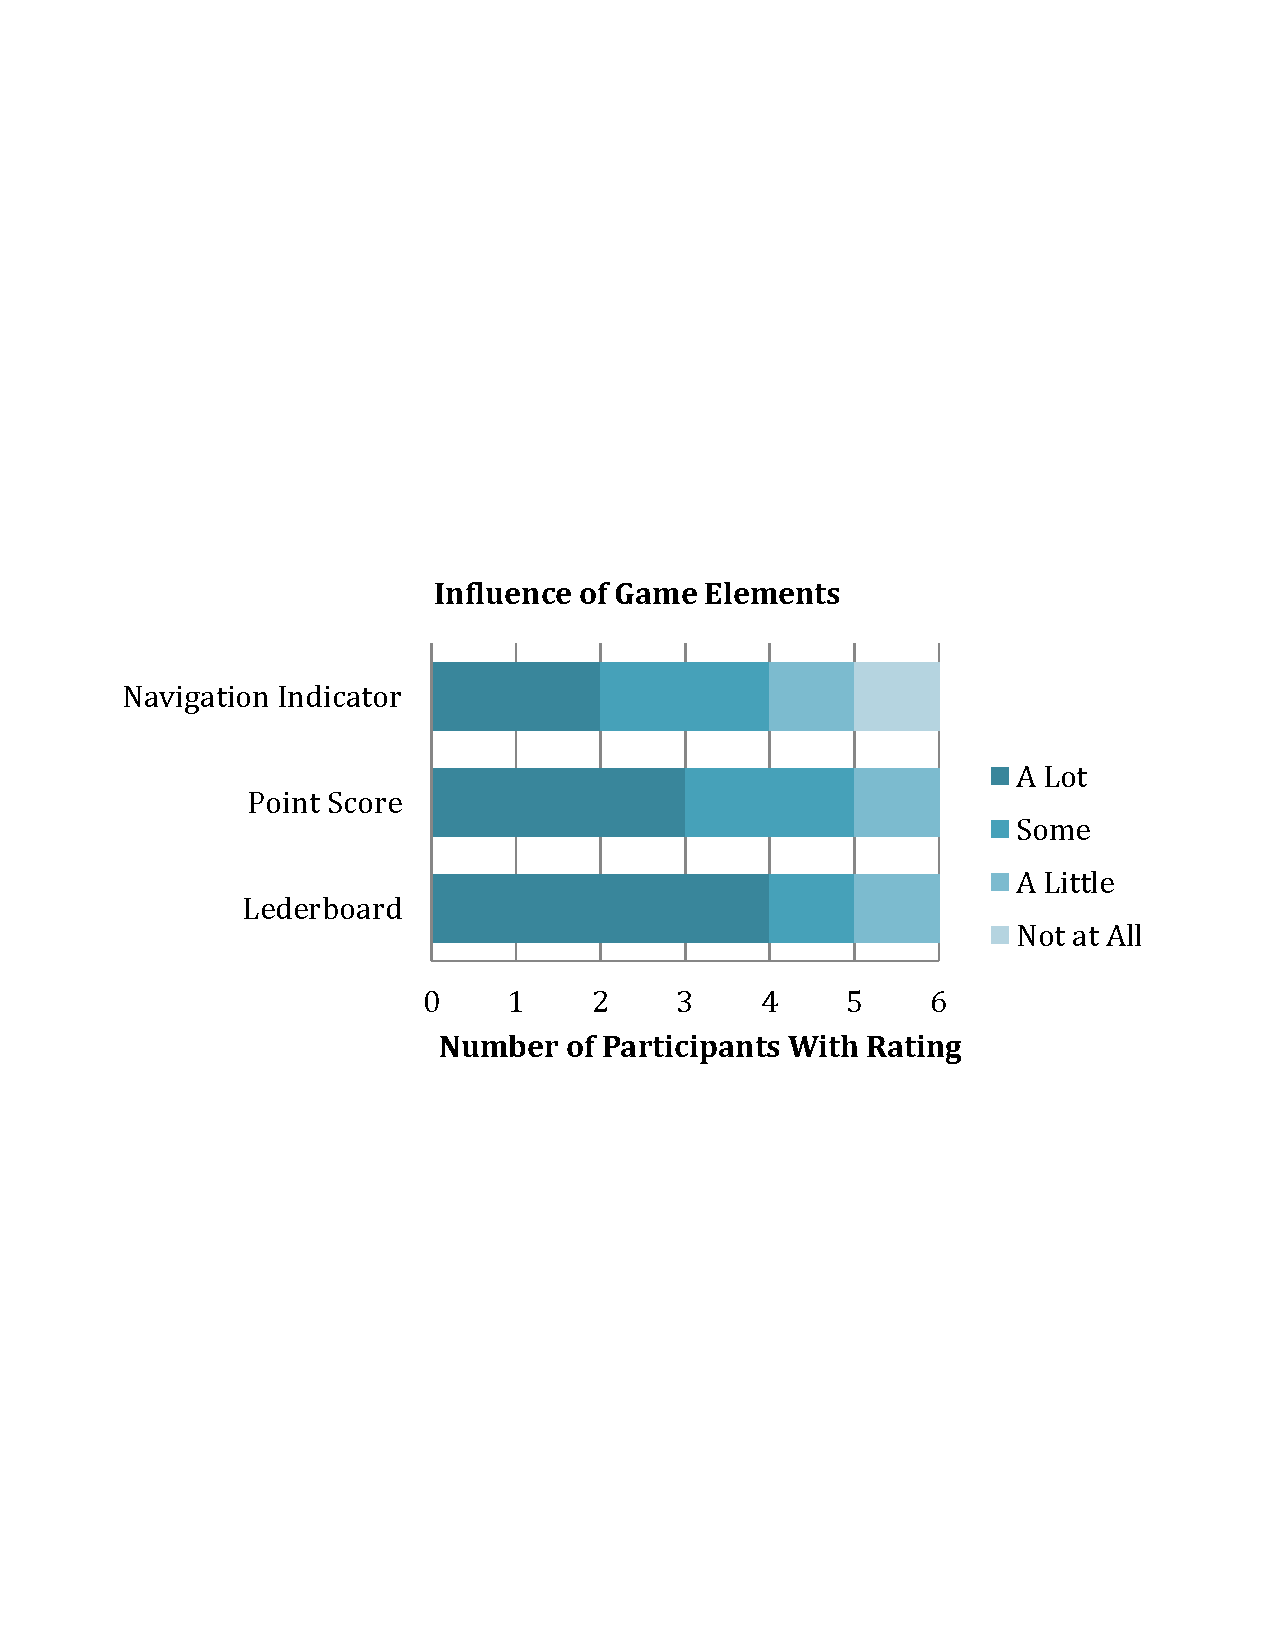
\includegraphics[width=3.4in]{ElementInfluenceChart.pdf}
	\caption{Influence of Feedback Elements}
	\label{fig:elementInfluence}
\end{figure}

The chart in figure \ref{fig:elementInfluence} shows how the individual feedback features influenced developers to think about using structured navigation.  Four out of six developers said the leaderboard influenced them "a lot" and all rated the leaderboard as having some influence.  Three out of six  said their individual point score influenced them "a lot" and all said the score had some influence.  The element with mixed ratings was a graphical indicator on whether they were improving over past use of structured navigation commands.  The indicator received the influencing "a lot" rating from one participant and a "not at all" influence rating from one participant with the rest having some influence.  The results indicate the more obvious and more clearly comparative information in the leaderboard was the strongest influence for developers.

The participants requested that the system to provide more feedback on tips to help them increase their score. They indicated that more obvious feedback such as hints that pop-up when they launch the tool would help them more than passively provided information.  Their desire for personal metrics and historical views of the data encourages us that this detailed level of measurement and analysis is perceived as helpful.  Features to meet these requests are part of future work.    

\section{Threats to Validity}
There are several threats to validity for this result.  By making the purpose of our measurement and contest known although without details we may have triggered the participants to think about navigation commands they use before establishing a baseline.  We attempt to control for this by comparing the pilot participants' data to data from Blaze users who are knowledgeable Visual Studio developers but did not receive the interventions.  Another threat is the intact team represents people with different backgrounds and experience levels who may have established habits for navigating through source code.  We attempt to control for this by asking post survey questions of the participants about their familiarity with the code they work in and their experience levels.  The threat of non- generalizable of results remains particularly because the pilot was conducted within an intact team in a single industrial site in India. As the pre-study questionnaire shows, the developer's desirability for a gamification type of intervention vary by country.

\section{Conclusions}
Developers accept gamification ideas into their environment even when coupled with detailed development activity monitoring.   We identified specific concerns particularly around maintaining anonymity of the developer as their data are shared with other developers.  The participants' feedback indicates a desire for more instructional hints on how to succeed in the game similar to how real games provide hints when the user might be stuck.  Implementing a more comprehensive set of practices in the game would expand the usefulness of Blaze as a training tool.  Other ideas might include making the game more subtle so that it is not as obvious a competition, but builds the elements of self-improvement that move the experience from an extrinsically motivated one to an intrinsically motivated one.  
%\end{document}  % This is where a 'short' article might terminate

%ACKNOWLEDGMENTS are optional
\section{Acknowledgments}
The authors wish to thank ABB and the pilot participants for their support of this research.

%
% The following two commands are all you need in the
% initial runs of your .tex file to
% produce the bibliography for the citations in your paper.
\bibliographystyle{abbrv}
\balance
\bibliography{../mousetap} 
 % sigproc.bib is the name of the Bibliography in this case
% You must have a proper ".bib" file
%  and remember to run:
% latex bibtex latex latex
% to resolve all references
%
% ACM needs 'a single self-contained file'!
%

\end{document}
